% Template for APA submission with R Markdown

% Stuff changed from PLOS Template
\documentclass[a4paper,man,apacite,floatsintext,longtable]{apa6}
\usepackage{apacite}

% amsmath package, useful for mathematical formulas
\usepackage{amsmath}
% amssymb package, useful for mathematical symbols
\usepackage{amssymb}

% hyperref package, useful for hyperlinks
\usepackage{hyperref}

% graphicx package, useful for including eps and pdf graphics
% include graphics with the command \includegraphics
\usepackage{graphicx}

% Sweave(-like)
\usepackage{fancyvrb}
\DefineVerbatimEnvironment{Sinput}{Verbatim}{fontshape=sl}
\DefineVerbatimEnvironment{Soutput}{Verbatim}{}
\DefineVerbatimEnvironment{Scode}{Verbatim}{fontshape=sl}
\newenvironment{Schunk}{}{}
\DefineVerbatimEnvironment{Code}{Verbatim}{}
\DefineVerbatimEnvironment{CodeInput}{Verbatim}{fontshape=sl}
\DefineVerbatimEnvironment{CodeOutput}{Verbatim}{}
\newenvironment{CodeChunk}{}{}

% cite package, to clean up citations in the main text. Do not remove.
\usepackage{cite}

\usepackage{color}

% Use doublespacing - comment out for single spacing
%\usepackage{setspace}
%\doublespacing


% Text layout
\topmargin 0.0cm
\oddsidemargin 0.5cm
\evensidemargin 0.5cm
\textwidth 16cm
\textheight 21cm

% Bold the 'Figure #' in the caption and separate it with a period
% Captions will be left justified
\usepackage[labelfont=bf,labelsep=period,justification=raggedright]{caption}


% Remove brackets from numbering in List of References
\makeatletter
\renewcommand{\@biblabel}[1]{\quad#1.}
\makeatother


% Leave date blank
\date{}

%\pagestyle{myheadings}
%% ** EDIT HERE **


%% ** EDIT HERE **
%% PLEASE INCLUDE ALL MACROS BELOW

%% END MACROS SECTION


% ALL OF THE TITLE PAGE INFORMATION IS SPECIFIED IN THE YAML
\title{\textbf{Developmental and postural changes in children's visual access to faces}}
\shorttitle{Children's visual access to faces}

\author{Michael C. Frank, Guido Pusiol, Daniel Yurovsky, Kaia Simmons}

\affiliation{Department of Psychology, Stanford University}

\authornote{Thanks to Ally Kraus, Kathy Woo, Aditi Maliwal, and other members of the
Language and Cognition Lab for help in recruitment, data collection, and
annotation. This research was supported by a John Merck Scholars grant
to MCF. An earlier version of this work was presented to the Cognitive
Science Society in Michael C Frank, Simmons, Yurovsky, \& Pusiol (2013).
Please address correspondence to Michael C. Frank, Department of
Psychology, Stanford University, 450 Serra Mall (Jordan Hall), Stanford,
CA, 94305, tel: (650) 724-4003, email:
\href{mailto:exttt\%7Bmcfrank@stanford.edu\%7D}{\nolinkurl{exttt\{mcfrank@stanford.edu\}}}.}
\abstract{The faces of other people are a critical information source for young
children. During early development, children undergo significant
postural and locomotor development, changing from lying and sitting
infants to toddlers who walk independently. We used a head-mounted
camera in conjunction with a face-detection system to explore the eff
ects of these changes on children's visual access to their caregivers'
faces during an in-lab play session. In a cross-sectional sample of
8--16 month old children, we found substantial changes in face
accessibility based on age and posture. These changes may translate into
changes in the accessibility of social information during language
learning. We make our corpus available for reanalysis, and discuss
strengths and limitations of the headcam method more generally.}
\keywords{social cognition; face-perception; infancy; locomotion; head-cameras}

\begin{document}
\maketitle

The ability to follow social signals like eye-gaze is an important part
of early social cognition (Scaife \& Bruner, 1975; M. Tomasello, 2009)

In addition to being an important part of early social development, the
ability to follow gaze is a strong predictor of children's early
language development. For example, Brooks \& Meltzoff (2005) found that
children who followed an experimenter's gaze better before their first
birthday had larger vocabularies at 18 months. Similarly, Carpenter,
Nagell, \& Tomasello (1998) found that children's level of joint
engagement (as well as the degree to which mothers followed the child's
focus of attention in their labeling) predicted vocabulary growth in
both language production and comprehension. These studies suggest that
children's social environment plays a powerful supportive role in
language learning.

But at the same time as children are beginning to learn their first
words, their view of the world is changing radically (Adolph \& Berger,
2007). As speechless infants, they are unable to locomote independently.
Before their first birthday, they begin crawling; soon after, they begin
to walk independently. Infants' visual field is subject to the whims of
their caregivers, but caregivers often place them in positions conducive
to joint attention. In contrast, toddlers determine their own input to a
much greater degree, but as a consequence they spend much of their time
in a world primarily populated by knees. These postural and locomotor
changes may have a profound effect on what children see.

A recent study suggests the possibility of links between motor
milestones, social cognition, and language. Walle \& Campos (2014) noted
robust correlations between children's ability to walk and their
vocabulary, both receptive and productive. On the basis of an
observational study of parent input, they speculated that the emergence
of walking may change the ability of the child to access social
information (because walking toddlers see more of the social world than
crawling infants). Accessing more social information may in turn allow
children to discover word meanings more effectively.

Recent methodological developments have the potential to provide data
that would allow this hypothesis to be tested. The availability of
head-mounted cameras and eye-trackers allows for the measurement of
children's naturalistic environment in a way that was not previously
possible. Yoshida \& Smith (2008) gave the first demonstration of the
radical differences between toddler and adult perspectives on the social
world, with toddlers' visual field being dominated by hands and objects
much more than that of adults. More recent work has used head-mounted
eye-tracking methods to measure young toddlers' fixations (Franchak,
Kretch, Soska, \& Adolph, 2011), also finding that children look
relatively infrequently at their mothers' faces in naturalistic play.

These methods are now being applied to understand inputs to language
acquisition. Work by Yu, Smith, and colleagues suggests that word
learning is facilitated when parents and children create moments in
which the visual field is dominated by a single object (L. B. Smith, Yu,
\& Pereira, 2011; Yu \& Smith, in press). Some data even suggest that
young children's restricted viewpoint may be more effective for learning
words than the comparable adult perspective (D. Yurovsky, Smith, \& Yu,
in press). Together, this body of evidence suggests that measuring
infants' perspective---and how it changes in motor development---is a
critical part of understanding early language learning.

In the current study we took a developmental approach to understanding
the relationship between perspective and access to social information.
We recorded head-camera data from a group of infants and children across
a broad age range as they played with their caregivers during a brief
laboratory visit. We then hand-annotated these data for the child's
posture and parents' naming behavior and used face-detection algorithms
to measure the frequency of faces in the child's visual field. The
resulting dataset allows us to analyze changes in access to faces
according to children's age, posture, and linguistic input.

\section{Methods}\label{methods}

\subsection{Participants}\label{participants}

\begin{table}[ht]
\centering
\begin{tabular}{rrrrrr}
  \hline
Age group & N & \% included & Mean age & Video length (min) & \% female \\ 
  \hline
  8 &  12 & 0.46 & 8.71 & 14.41 & 0.50 \\ 
   12 &  12 & 0.40 & 12.62 & 13.48 & 0.58 \\ 
   16 &  12 & 0.31 & 16.29 & 15.00 & 0.50 \\ 
   \hline
\end{tabular}
\caption{\label{tab:pop} Demographics by age group.}
\end{table}

Our final sample consisted of 36 infants and children, distributed into
each of three age groups: 8 months, 12 months, and 16 months.
Participants were recruited from the surrounding community via state
birth records. Participants had no documented disabilities and were
reported to hear at least 80\% English at home. Demographics and
exclusion rates are given in Table \ref{tab:pop}.

In order to compile this final sample, we tested a substantially larger
group of children, who were excluded for the following reasons: 20 for
technical issues related to the headcam, 15 for failing to wear the
headcam, 10 for fewer than 4 minutes of headcam footage, 5 for having
multiple adults present, 5 for missing CDI data, 2 for missing scene
camera footage, 1 for fussiness, and one excluded for sample symmetry.
All inclusion decisions were made independent of the results of
subsequent analyses.

\subsection{Head-mounted camera}\label{head-mounted-camera}

\begin{figure}
\centering
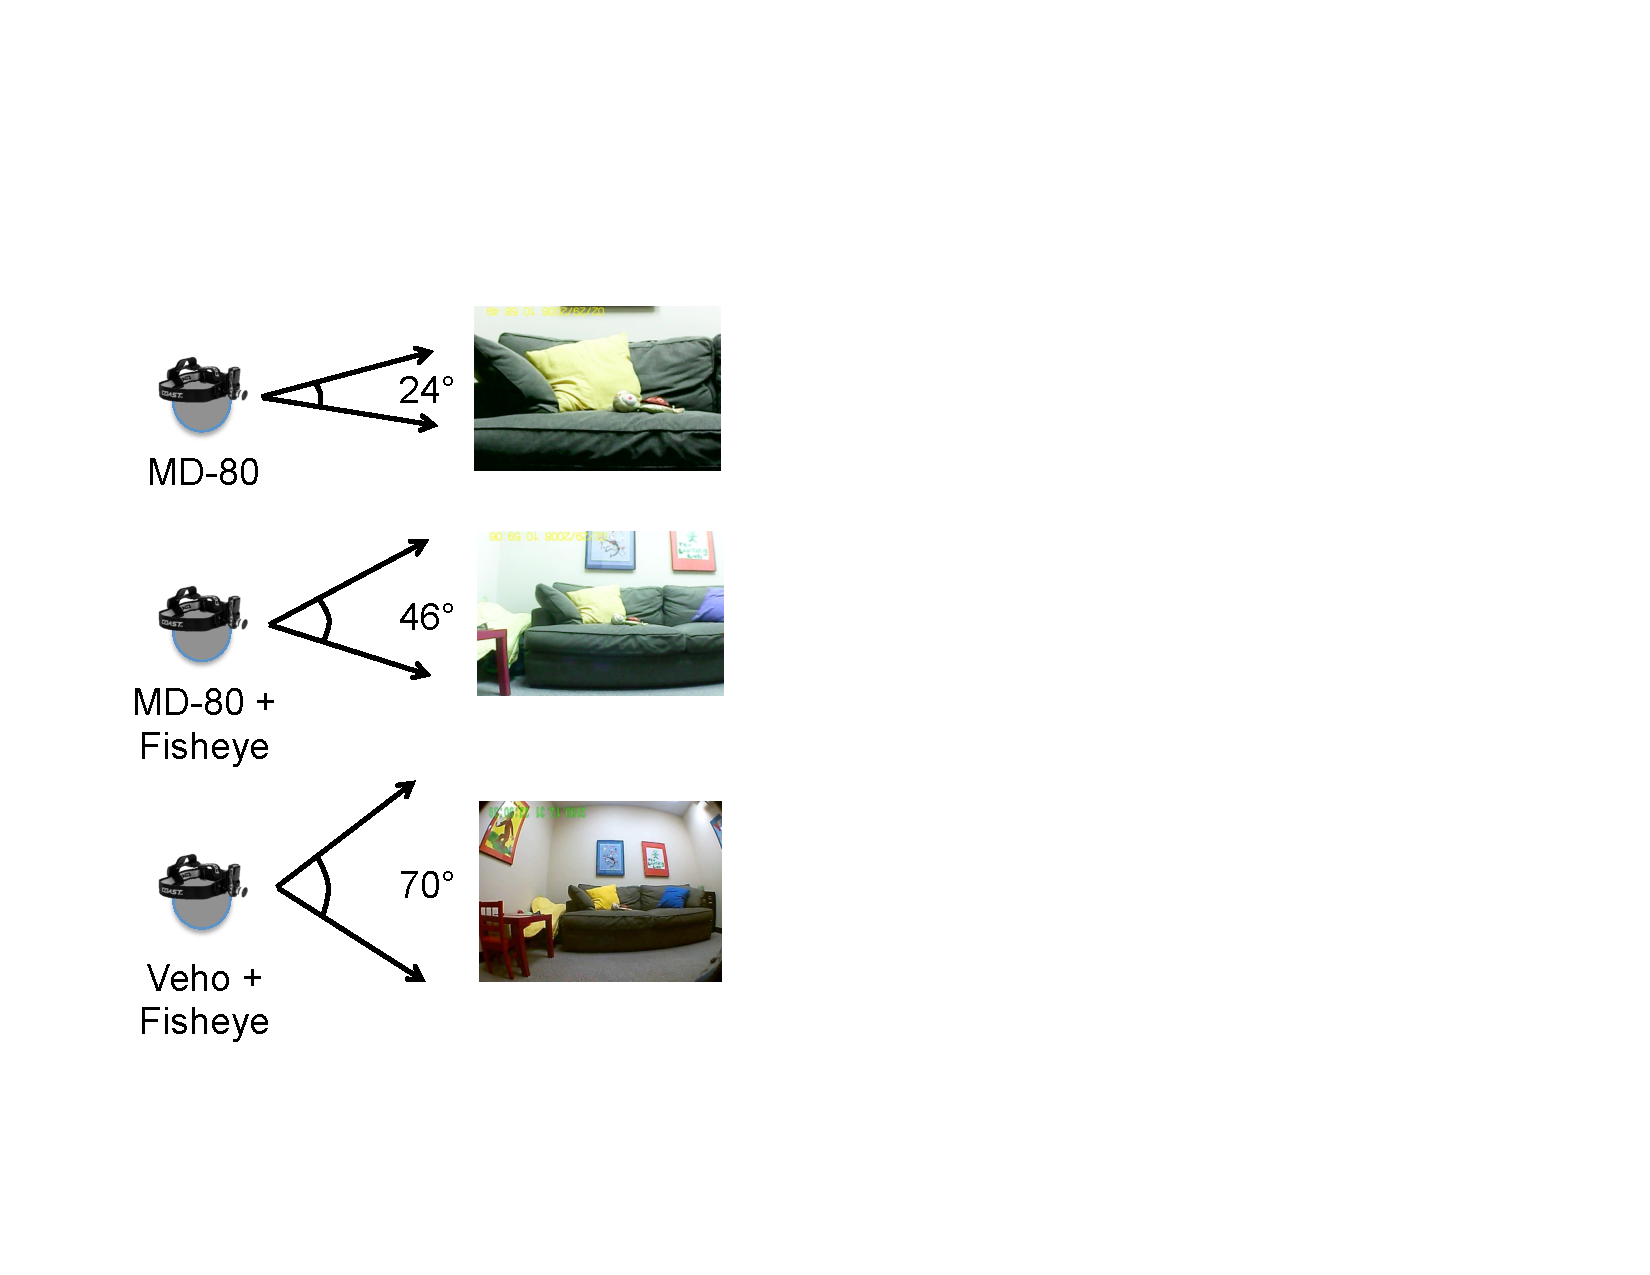
\includegraphics[width=3in]{images/viewangle.pdf}
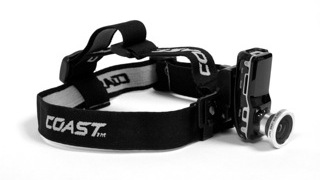
\includegraphics[width=2in]{images/headcam_w_fisheye3.jpg}
\caption{\label{fig:headcam} Left: Field of view for three different headcam configurations, with the device we used in the middle. The lowest camera is pictured for comparison, but was not available until after our study was already in progress. Right: The light-weight, low-cost head-mounted camera with fisheye lens.}
\end{figure}

Our head-mounted camera (``headcam'') is composed of a small,
inexpensive MD80 model camera attached to a soft elastic headband from a
camping headlamp. An aftermarket fisheye lens intended for iPhones and
other Apple devices is attached to increase view angle. The total cost
of each camera is approximately \$60. The camera captures 720x480 pixel
images at approx. 25 frames per second, and has battery life of 60--90
minutes. Without the fisheye lens, the viewing angle for the camera is
\(32^{\circ}\) horizontal by \(24^{\circ}\) vertical; with the fisheye,
\(64^{\circ}\) horizontal by \(46^{\circ}\) vertical (see Figure
\ref{fig:headcam}, left). The device is pictured in Figure
\ref{fig:headcam}, right. Instructions for creating the camera are given
in detail at
\url{http://babieslearninglanguage.blogspot.com/2013/10/how-to-make-babycam.html}.

The vertical field of view of the camera was considerably smaller than
the child's approximate vertical field of view, which---even at 6-7
months---spans around 100--120\(^{\circ}\) in the vertical dimension
(Cummings, Van Hof-Van Duin, Mayer, Hansen, \& Fulton, 1988; Mayer,
Fulton, \& Cummings, 1988). We were therefore faced with a choice in the
orientation of the camera. If we chose a lower or higher orientation, we
would be at risk of truncating either the child's own hands and
physically proximate objects, or the faces of the adults around the
child. Yet if we chose the middle orientation, we would still be at risk
of underestimating the proportion of faces viewed by the child. Thus,
for the purposes of the current study---measuring visual access to
faces---we chose to orient the camera towards the upper part of the
visual field. While this orientation decreased our chances of recording
the objects being manipulated by the child, it nevertheless allowed us
to capture the majority of the faces in the child's visual field.

\subsection{Procedure}\label{procedure}

Before coming to the lab, caregivers completed the MacArthur-Bates
Communicative Development Inventories Words and Gestures form (Fenson et
al., 2007), reporting on the words that they believed that their child
understood and produced.

After coming to the lab, families were seated in our waiting room where
they signed consent documents and where children were fitted with the
headcam. After a short period of play, they were escorted to a playroom
in the lab where the free-play session (the focus of the current study)
was conducted.

In the waiting room, the experimenter placed the headcam on children's
heads after they had time to adjust to the environment. For children who
resisted wearing the headcam, the experimenter used distractor
techniques (presenting stimulating toys or engaging the children in
hand-occupying activities) intended to keep children's focus elsewhere
and prevent them from taking off the camera (Yoshida \& Smith, 2008).
Once the child was wearing the camera comfortably for a period of time,
child and caregiver were escorted to the playroom.

In the playroom, the experimenter presented the child's parent with a
box containing three labeled pairs of objects, each consisting of a
familiar and a novel object (e.g.~a ball and a feather duster, marked as
a ``zem''). Parents confirmed that the child had not previously seen the
novel toys. Parents were instructed to play with the object pairs with
the child, one at a time, ``as they typically would'' and to use the
novel labels to refer to the three toys. After giving these
instructions, the experimenter left the room for a period of
approximately 15 minutes. During this time, a tripod-mounted camera
recorded video from a corner of the room and the headcam captured video
from the child's perspective.

\subsection{Data Processing and
Annotation}\label{data-processing-and-annotation}

\begin{figure*}

\includegraphics[width=6in]{images/framesample.pdf}
\caption{\label{fig:frames} Sample frames from the headcam videos for a child from each age group, selected because they featured successful face detections (green squares).}
\end{figure*}

All headcam videos were cropped to exclude the period of entry to the
playroom and were automatically synchronized with the tripod-mounted
videos using FinalCut Pro Software. These sessions yielded a substantial
amount of video: a total of 515 minutes (almost a milion frames), with
an average video length of 8.58 minutes (min = 4.53, max = 19.35).

\subsubsection{Posture and Orientation
Annotation}\label{posture-and-orientation-annotation}

One major goal of our study was to understand the relationship between
children's posture and their access to information from the faces of
their caregiver. To investigate this relationship, we created a set of
annotations for the child's physical posture (e.g.~standing, sitting)
and orientation of the caregiver relative to the child (e.g.~in front
of, behind, close, far away). For each headcam video, a coder used
OpenSHAPA software to annotate both orientation and posture (Adolph,
Gilmore, Freeman, Sanderson, \& Millman, 2012).

Orientation was initially categorized as having the caregiver in front,
to the side, or behind the child, and close (defined informally as
within arm's reach) or farther away. Because of data sparsity, we
consolidated this scheme into three categories: close to the caregiver
with the caregiver either in front or on the side, farther from the
caregiver again with caregiver either in front or on the side, and a
global category of caregiver behind the child. Posture was categorized
as being held/carried, lying face-up, sitting, prone (crawling or
lying), standing, or other. Data from when the child was out of view of
the tripod camera was marked as uncodable and excluded from these
annotations. \% A second coder coded XYZ videos; their categorizations
were reliable at XYZ.

\subsubsection{Labeling Annotation}\label{labeling-annotation}

We were also interested in the availability of social information
proximate to naming events in the caregivers' speech to children.
Accordingly, a human coder marked the onset time when the name of any of
the six objects in the object set was used. Overall, caregivers produced
a median of XYZ labels in a highly skewed distribution across
participants (range: XYZ -- XYZ).

\subsection{Face Detection}\label{face-detection}

An additional goal of the study was to measure the presence of
caregivers' faces in the child's field of view (as approximated by the
headcam). To avoid hand-annotating the size and position of faces in
every frame of video, we tested two face detection systems. Sample
frames from the video with successful detections are given in Figure
\ref{fig:frames}.

\subsubsection{Face detection
algorithms}\label{face-detection-algorithms}

The first algorithm was based on freely available computer vision tools
(Bradski \& Kaehler, 2008) and is described in depth in our previous
work (M. C. Frank, 2012). This system had two parts. The first was the
application of a set of four Haar-style face detection filters (Viola \&
Jones, 2004) to each frame of the videos independently. These detectors
each provide information about whether a face is present in the frame as
well as size and position for any detections. In a second step, these
detections are then combined via a hidden Markov model (HMM), trained on
hand-annotated data (see Appendix). The HMM model (which performed
nearly as well as the more complex and computationally-intensive
Conditional Random Field model used in our previous work) attempted to
estimate whether a face was truly present in each frame of the videos,
using as its input the number of Haar detectors that were active in any
given frame.

The second algorithm that we evaluated was a semi-automated adaptive
tracker-by-detection (SAATD). The algorithm required manual user input
(selecting a single face example per video) for its initialization, but
then needed no additional training data. The tracker is based on Kalal,
Mikolajczyk, \& Matas (2010), which uses patches in the trajectory of an
optical-flow based tracker (Lucas \& Kanade, 1981) to train and update a
face detector. The optical flow tracker and the face detector work in
parallel.

\subsubsection{Detector evaluation}\label{detector-evaluation}

\begin{table}[t]
  \caption{Model performance on gold standard generalization training set dataset. P, R, and F denote precision, recall, and F-score for each of the two samples. \label{tab:model_eval}}
  \begin{center}
    \begin{tabular}{l|ccc|ccc}
      \hline
       &  \multicolumn{3}{c|}{High-density} &  \multicolumn{3}{c}{Random} \\
      % \null Model & P & R & F & P & R & F  \\
      \hline
      % HMM & .55  & .38 &  .45 & .89 & .74 & .81   \\
      % SAATD & .86 & .78 & .81 & .93 & .76 & .83 \\
    \hline
    \end{tabular}
  \end{center}
\end{table}

To ensure that our evaluation was not biased by the relatively rare
appearance of faces in the dataset, we annotated two samples, both a
random sample from the data and a sample with a high-density of faces.
We selected 1 minute of interaction for each age group, divided evenly
across the four dyads at that age. For each dyad, we divided the
recorded video into contiguous 1 s segments and selected 16 in
accordance with two criteria. First, 8 of these segments were selected
by choosing the parts of the videos highest in face detection
(\emph{high density sample}). To be fair to both algorithms, half of
this was chosen from the segments with the most HMM detections and half
were chosen from the segments with the most SAATD detections. The
remaining segments were chosen by randomly sampling from segments not
yet selected for coding (\emph{random sample}).

Segments were annotated frame-by-frame by a human coder, who marked each
frame as containing a face if at least half of the face was in the
child's view. Detector output for each of these frames was then compared
to this gold standard. A detection was counted as correct if it
overlapped a face with half of its total area. The HMM training sample
was selected via the same method as this gold standard sample, but used
separate set of video segments.

We evaluated each algorithm on its precision (hits / hits + false
alarms) and recall (hits / hits + misses), as well as F-score (the
harmonic mean of these two measures). Results are reported in Table
\ref{tab:model_eval}.

The HMM model obtained a relatively high level of performance for the
random subsections, but performed poorly when there was a relatively
high density of faces present. In contrast, SAATD performed well on both
samples, giving better performance especially in cases where there was
partial occlusion. Our goal in using face-detection algorithms was to
provide a measurement technique that eliminated tedious and expensive
hand-coding and provided acceptable results. We therefore selected the
SAATD model and report detections from this algorithm as an estimate of
face presence in all further analyses.

\section{Results}\label{results}

We report results from three different sets of analyses. First, we
explore developmental changes in posture and orientation in our dataset.
Next, we explore how these changes affect access to faces, as measured
using our face-detection algorithm. Finally, we report preliminary
results on the accessibility of faces during labeling.

\subsection{Changes in Posture and
Orientation}\label{changes-in-posture-and-orientation}

Our posture coding captured typical developmental milestones (Figure
\ref{fig:posture}). Overall, sitting was the most common posture for
interactions in the caregiver play session. The youngest infants in our
sample mostly sat (with parental assistance), but also lay down and were
carried a significant proportion of the time. The 12-month-olds were the
only group who spent a large amount of time crawling, and the 16- and
20-month-olds sat and stood in equal parts.

Similarly, our coding of orientation revealed some significant
developmental changes (Figure \ref{fig:orientation}). Younger children
more frequently had the caregiver behind them, often because the
caregiver was supporting the child's sitting posture (for the
4-month-olds especially). In contrast, the 12--20 month olds were able
to locomote independently and so were able to spend more time further
from the caregiver.

\subsection{Access to Faces}\label{access-to-faces}

We next investigated the effects of the child's posture and orientation
on the presence and size of the caregiver's face in the visual field.
Figure \ref{fig:face_dets} shows the proportion of frames with a
positive face detection, plotted by the child's age, posture, and
orientation relative to the caregiver.

Overall, there were very large differences in access to faces across
age. The 4-month-olds saw almost no faces---their parents were behind
them most of the time, supporting them since they could not sit
independently. In contrast, the 8-month-olds, who could sit
independently, typically sat across from their caregiver and saw many
faces in both the sitting and prone postures. The 12-month-olds spent a
large amount of time in the prone position (typically crawling after the
ball, for example) and saw almost no faces in that posture. The 16- and
20-month-olds saw many faces because they were standing while their
parents were sitting, putting their faces at a relatively similar level.

Across ages, the carrying and prone postures resulted in the smallest
number of faces seen, while standing and sitting resulted in far more.
These postures both presented opportunities for seeing faces in large
part because parents were sitting or lying on the floor with children.
Although far fewer faces were seen when the caregiver was behind the
child,\footnote{Since orientation was coded via body posture, faces seen
  while the caregiver was behind the child were due to children looking
  over their shoulder.} both the close and far positions resulted in
approximately equal proportions of face detections.

\subsection{Access to Faces During
Labeling}\label{access-to-faces-during-labeling}

Our final analysis concerned the accessibility of caregivers' faces
during labeling events. Franchak et al. (2011) found that referential
speech was marginally more likely to draw toddlers' attention to
mothers' faces. We were similarly interested in whether looking at faces
occurred during labeling. Accordingly, we used the labeling annotations
for each child to identify the 2s before and after each labeling event.
We then computed the proportion face detections within this window
across ages.

The overall pattern of face accessibility closely mirrored the base
rates shown in Figure \ref{fig:face_dets}. Although this general pattern
in itself is important in assessing developmental access to social
information, in the current analysis we were interested in whether there
was differential access to faces around labeling instances. We thus
computed difference scores between the baseline face detection rate and
the rate of face detections in labeling windows for each participant.
Figure \ref{fig:naming_face} shows the results of this analysis.

Although any conclusion must remain extremely tentative because of the
small sample, we nevertheless saw an increase in label-related face
access for the 20-month-olds. This difference was robust across a
variety of window sizes from 1--6 s. (8-month-olds were more variable
but similarly showed some trend towards greater face access during
naming.) We cannot yet make inferences about the source of these
differences: They could be could be caused by children, caregivers, or a
combination of the two. Nevertheless, these results converge with
previous work and suggest that, in combination with face detection
techniques, the headcam may be a viable method for examining social
access during language learning.

\section{General Discussion}\label{general-discussion}

Using a head-mounted camera, we explored the relationship between
infants' postural and locomotor development and their visual access to
social information. The use of automated annotation tools from computer
vision allowed us to measure the prevalence of caregivers' faces in
their children's visual field. We found systematic differences in the
visual accessibility of faces based on posture, orientation, and age, as
well as hints of differences in language-related changes in visual
access. While these results remain preliminary given the size of our
developmental sample, this work nevertheless provides an important
proof-of-concept that computer vision techniques can be used as a
measurement method in the developmental context.

The measures developed here have broad applicability to the study of
individual and cultural differences. Since the physical circumstances of
child rearing vary widely across households and across cultures, there
may be important and predictable differences in children's visual
experience. As suggested by the correlations between walking and
vocabulary development ({\textbf{???}}), postural development may have
substantial downstream consequences for language. For example, shifts in
how infants are placed in particular postures by strollers or carriers
(Zeedyk, 2008) or how their motor development is encouraged by parent
practices (Bril \& Sabatier, 1986) may lead to differences in social
input which in turn affect their language learning. Since our variant of
the headcam method is both inexpensive and highly portable, we have been
able to deploy it in children's homes with some success; it may thus be
a valuable tool for investigating differences in child-rearing
practices.

A deep body of work uses children's linguistic input---measured using
audio recordings---to understand the learning mechanisms underlying
vocabulary acquisition (Fernald, Perfors, \& Marchman, 2006; Hart \&
Risley, 1995; Huttenlocher, Haight, Bryk, Seltzer, \& Lyons, 1991).
There have been some important initial successes in using visual input
to predict language uptake (Yu \& Smith, in press). Nevertheless, we
have a long way to go before our knowledge about children's visual input
parallels our understanding of their linguistic environment. Coming to
such an understanding will require the creation of both corpus resources
and automated tools such as those we have begun to develop here.

\section{View angle}\label{view-angle}

We note that previous studies have shown that children's head movements
in the horizontal dimension are approximated by (though are slightly
lagged by) their head movements (Yoshida \& Smith, 2008). Our own
experience with the current apparatus ratifies these conclusions for the
horizontal field but suggests that head movements in the vertical field
are less reliable. Hence, these studies may run the risk of
underestimating the proportion of faces actually seen by children.

\section*{References}\label{references}
\addcontentsline{toc}{section}{References}

\hypertarget{refs}{}
\hypertarget{ref-adolph2007}{}
Adolph, K., \& Berger, S. (2007). Motor development. In \emph{Handbook
of child psychology}. Wiley Online Library.

\hypertarget{ref-adolph2012}{}
Adolph, K., Gilmore, R., Freeman, C., Sanderson, P., \& Millman, D.
(2012). Toward open behavioral science. \emph{Psychological Inquiry},
\emph{23}(3), 244--247.

\hypertarget{ref-bradski2008}{}
Bradski, G., \& Kaehler, A. (2008). \emph{Learning OpenCV: Computer
vision with the OpenCV library}. O'Reilly Media.

\hypertarget{ref-bril1986}{}
Bril, B., \& Sabatier, C. (1986). The cultural context of motor
development: Postural manipulations in the daily life of Bambara babies
(Mali). \emph{International Journal of Behavioral Development},
\emph{9}(4), 439--453.

\hypertarget{ref-brooks2005}{}
Brooks, R., \& Meltzoff, A. (2005). The development of gaze following
and its relation to language. \emph{Developmental Science}, \emph{8}(6),
535--543.

\hypertarget{ref-carpenter1998}{}
Carpenter, M., Nagell, K., \& Tomasello, M. (1998). Social cognition,
joint attention, and communicative competence from 9 to 15 months of
age. \emph{Monographs of the Society for Research in Child Development},
\emph{63}(4).

\hypertarget{ref-cummings1988}{}
Cummings, M., Van Hof-Van Duin, J., Mayer, D., Hansen, R., \& Fulton, A.
(1988). Visual fields of young children. \emph{Behavioural and Brain
Research}, \emph{29}(1), 7--16.

\hypertarget{ref-fenson2007}{}
Fenson, L., Bates, E., Dale, P. S., Marchman, V. A., Reznick, J. S., \&
Thal, D. J. (2007). \emph{MacArthur-bates communicative development
inventories: Users manual}. Brookes Publishing Company.

\hypertarget{ref-fernald2006}{}
Fernald, A., Perfors, A., \& Marchman, V. (2006). Picking up speed in
understanding: Speech processing efficiency and vocabulary growth across
the 2nd year. \emph{Developmental Psychology}, \emph{42}(1), 98--116.

\hypertarget{ref-franchak2011}{}
Franchak, J., Kretch, K., Soska, K., \& Adolph, K. (2011). Head-mounted
eye tracking: A new method to describe infant looking. \emph{Child
Development}.

\hypertarget{ref-frank2012b}{}
Frank, M. C. (2012). Measuring children's visual access to social
information using face detection. In \emph{Proceedings of the 33nd
Annual Meeting of the Cognitive Science Society}.

\hypertarget{ref-frank2013}{}
Frank, M. C., Simmons, K., Yurovsky, D., \& Pusiol, G. (2013).
Developmental and postural changes in children’s visual access to faces.
In \emph{Proceedings of the 35th annual meeting of the cognitive science
society} (pp. 454--459).

\hypertarget{ref-hart1995}{}
Hart, B., \& Risley, T. (1995). \emph{Meaningful differences in the
everyday experience of young American children}. Baltimore, MD: Brookes
Publishing Company.

\hypertarget{ref-huttenlocher1991}{}
Huttenlocher, J., Haight, W., Bryk, A., Seltzer, M., \& Lyons, T.
(1991). Early vocabulary growth: Relation to language input and gender.
\emph{Developmental Psychology}, \emph{27}(2), 236--248.

\hypertarget{ref-kalal2010}{}
Kalal, Z., Mikolajczyk, K., \& Matas, J. (2010). Forward-backward error:
Automatic detection of tracking failures. In \emph{20th International
Conference on Pattern Recognition} (pp. 2756--2759). IEEE.

\hypertarget{ref-lucas1981}{}
Lucas, B., \& Kanade, T. (1981). An iterative image registration
technique with an application to stereo vision. In \emph{Proceedings of
the 7th International Joint Conference on Artificial intelligence}.

\hypertarget{ref-mayer1988}{}
Mayer, D., Fulton, A., \& Cummings, M. (1988). Visual fields of infants
assessed with a new perimetric technique. \emph{Investigative
Ophthalmology \& Visual Science}, \emph{29}(3), 452--459.

\hypertarget{ref-scaife1975}{}
Scaife, M., \& Bruner, J. (1975). The capacity for joint visual
attention in the infant. \emph{Nature}, \emph{253}, 265--266.

\hypertarget{ref-smith2011}{}
Smith, L. B., Yu, C., \& Pereira, A. F. (2011). Not your mother's view:
The dynamics of toddler visual experience. \emph{Developmental Science},
\emph{14}, 9--17.

\hypertarget{ref-tomasello2009}{}
Tomasello, M. (2009). \emph{The cultural origins of human cognition}.
Harvard University Press.

\hypertarget{ref-viola2004}{}
Viola, P., \& Jones, D. H. (2004). Robust real-time face detection.
\emph{International Journal of Computer Vision}.

\hypertarget{ref-walle2014}{}
Walle, E. A., \& Campos, J. J. (2014). Infant language development is
related to the acquisition of walking. \emph{Developmental Psychology},
\emph{50}(2), 336.

\hypertarget{ref-yoshida2008}{}
Yoshida, H., \& Smith, L. (2008). What's in view for toddlers? Using a
head camera to study visual experience. \emph{Infancy}, \emph{13},
229--248.

\hypertarget{ref-yuinpress}{}
Yu, C., \& Smith, L. B. (in press). Embodied attention and word learning
by toddlers. \emph{Cognition}.

\hypertarget{ref-yurovsky2012}{}
Yurovsky, D., Smith, L., \& Yu, C. (in press). Statistical word learning
at scale: The baby's view is better. \emph{Developmental Science}.

\hypertarget{ref-zeedyk2008}{}
Zeedyk, M. (2008). \emph{What's life in a baby buggy like?: The impact
of buggy orientation on parent-infant interaction and infant stress}.
London, UK: National Literacy Trust.

\bibliography{xsface.bib}

\end{document}
